\chapter{Graphs and gating functions \Author{J. Stanier}}
\label{chapter:vsdg}
\inputpath{part2}{vsdg}
\inputprogress


\newcommand{\Gn}{$\gamma$-node}
\newcommand{\Gns}{$\gamma$-nodes}
\newcommand{\Tn}{$\theta$-node}
\newcommand{\Tns}{$\theta$-nodes}
\newcommand{\Ttns}{$\theta^{\mathit{tail}}$-nodes}
\newcommand{\triVM}{\textit{tri}VM}

\newcommand{\instruction}[1]{\texttt{#1}}
\newcommand{\register}[1]{\texttt{v#1}}

\section{Introduction}
Many compilers represent the input program as some form of graph in order to aid analysis and transformation. 
A cornucopia of program graphs has been presented in the literature and implemented in real compilers. 
Therefore it comes as no surprise that a number of program graphs use SSA concepts as the core principle of their representation. 
These range from very literal translations of SSA into graph form to more abstract graphs which are implicitly SSA. 
We aim to introduce a selection of program graphs which use SSA concepts, and examine how they may be useful to a compiler writer.

One of the seminal graph representations is the Control-Flow Graph (CFG), which was introduced by Allen to explicitly represent possible control paths in a program. 
Traditionally, the CFG is used to convert a program into SSA form. 
Additionally, representing a program in this way makes a number of operations simpler to perform, such as identifying loops, discovering irreducibility and performing interval analysis techniques.

The CFG models control flow, but many graphs model \textit{data flow}. 
This is useful as a large number of compiler optimizations are based on data flow. 
The graphs we consider in this chapter are all data-flow graphs, representing the data dependencies in a program. 
We will look at a number of different SSA-based graph representations. 
These range from those which are a very literal translation of SSA into a graph form to those which are more abstract in nature. 
An introduction to each graph will be given, along with diagrams to show how sample programs look when translated into that particular graph. 
Additionally, we will touch on the literature describing a usage of a given graph with the application that it was used for.

\section{Data-flow Graphs}

The data-flow graph (DFG) is a directed graph $G=(V,E)$ where the edges $E$ represent the flow of data from the result of one operation to the input of another. 
An instruction executes once all of its input data values have been consumed. 
When an instruction executes, it produces a new data value which is propagated to other connected instructions.

Whereas the CFG imposes a total ordering on instructions, the DFG has no such concept, nor does the DFG contain whole program information. 
Thus, target code cannot be generated directly from the DFG. 
The DFG can be seen as a companion to the CFG, and they can be generated alongside each other. 
With access to both graphs, optimizations such as dead code elimination, constant folding and common subexpression elimination can be performed effectively. 
However, keeping both graphs updated during optimization can be costly and complicated.

\section{The SSA Graph}

We begin our exploration with a graph that is very similar to SSA: 
the SSA Graph. 
Notice that many different variations exist in the literature. 
For us, an SSA Graph consists of vertices which represent operations (such as \texttt{add} and \texttt{load}) or \phifuns, and directed edges connect uses to definitions of values. 
The outgoing edges from a vertex represent the arguments required for that operation, and the ingoing edge(s) to a vertex represents the propagation of that operation's result(s) after it has been computed. 
This graph is therefore a \textit{demand-based} representation. 
In order to compute a vertex, we must first \textit{demand} the results of the operands and then perform the operation indicated on that vertex. 
Reversing the direction of each edge would provide the widely used \emph{data-based} representation. 
The SSA Graph can be constructed from a program in SSA form by \textit{explicitly} adding use-definition chains. 
We present some sample code in Figure~\ref{fig: 
  ssa-graph-example-code} which is then translated into an SSA Graph.
%FAB: I do not see any motivation for not representing the full operation in each of the node as done by Florian in the propagation engine chapter.
%% Note that there are no explicit nodes for variables in the graph. Instead, an operator node can be seen as the ``location'' of the value stored in a variable. We have annotated operators with variable names to show the correspondence between the operations in the graph and in the SSA form program.
Note that each node mixes up the operation and the variable(s) it defines, as actual data structures might be able to find one from the other.

\begin{figure}[ht]
\centering
\subfloat{
  \begin{minipage}[b]{0.3\linewidth}
    \texttt{\begin{tabbing}
	begin: \=$a_{0}$ = 0; \\
	\> $i_{0}$ = 0; \\
	loop: \> $a_{1}$ = $\phi$($a_{0}$,$a_{2}$); \\
	\> $i_{1}$ = $\phi$($i_{0}$,$i_{2}$); \\
        \> if $i_1$ > 100 goto end; \\
	\> $a_{2}$ = $a_{1}$ * $i_{1}$; \\
	\> $i_{2}$ = $i_{1}$ + 1; \\
	\> if $a_2$ > 20 goto end;\\
        \> goto loop;\\
	end: \> $a_{3}$ = $\phi$($a_{1}$,$a_{2}$); \\
	\> $i_{3}$ = $\phi$($i_{1}$,$i_{2}$); \\
	\> print($a_{3}$ + $i_{3}$);
      \end{tabbing}}
  \end{minipage}
}
\subfloat{
  \begin{minipage}[b]{0.3\linewidth}
    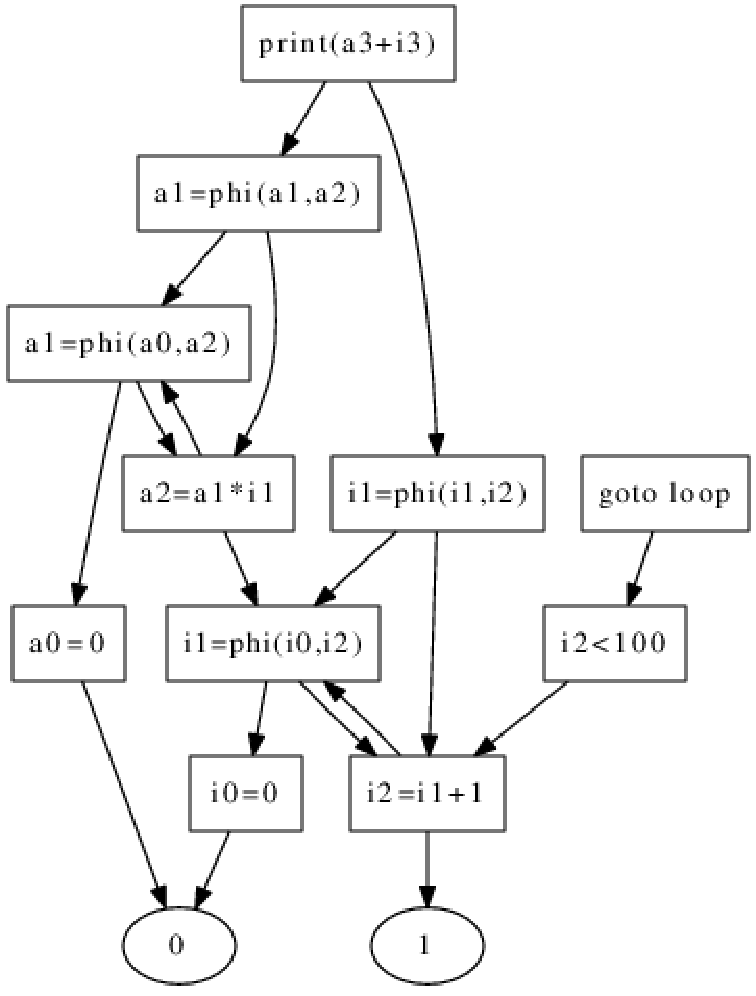
\includegraphics[scale=0.5]{ssa-graph-2.pdf}
  \end{minipage}
}

\caption{Some SSA code translated into a (demand-based) SSA graph.}
\label{fig: ssa-graph-example-code}
\end{figure}

The textual representation of SSA is much easier for a human to read. 
However, the primary benefit of representing the input program in this form is that the compiler writer is able to apply a wide array of graph-based optimizations by using standard graph traversal and transformation techniques. 
It is possible to augment the SSA Graph to model memory dependencies. 
This can be achieved by adding \textit{state edges} that enforce an order of interpretation. 
These edges are extensively used in the Value State Dependence Graph, which we will look at later, after we touch on the concept of gating functions.

In the literature, the SSA Graph has been used to detect a variety of induction variables in loops, also for performing instruction selection techniques, operator strength reduction, rematerialization, and has been combined with an extended SSA language to aid compilation in a parallelizing compiler. 
The reader should note that the exact specification of what constitutes an SSA Graph changes from paper to paper. 
The essence of the intermediate representation (IR) has been presented here, as each author tends to make small modifications for their particular implementation.

\subsection{Finding induction variables with the SSA Graph}
We illustrate the usefulness of the SSA Graph through a basic induction variable (IV) recognition technique. 
A more sophisticated technique is developed in Chapter~\ref{chapter:loop_tree}. 
Given that a program is represented as an SSA Graph, the task of finding induction variables is simplified. 
A \textit{basic linear induction variable} $i$ is a variable that appears only in the form:

\begin{center}
  \begin{minipage}[b]{0.3\linewidth}
    \texttt{\begin{tabbing}
         i = 10\\
         loop \=\\
         \> ...\\
         \> i = i + k\\
         \> ...\\
         endloop
      \end{tabbing}}
  \end{minipage}
\end{center}

where $k$ is a constant or loop invariant. 
A simple IV recognition algorithm is based on the observation that each basic linear induction variable will belong to a non-trivial strongly connected component (SCC) in the SSA graph. 
SCCs can be easily discovered in linear time using any depth first search traversal. 
Each such SCC must conform to the following constraints:

\begin{itemize}
\item The SCC contains only one \phifun at the header of the loop.
\item The SCC contains only addition and subtraction operators, and the right operand of the subtraction is not part of the SCC (no \texttt{i=n-i} assignments).
\item The other operand of each addition or subtraction is loop invariant.
\end{itemize}

This technique can be expanded to detect a variety of other classes of induction variables, such as wraparound variables, non-linear induction variables and nested induction variables. 
Scans and reductions also show a similar SSA Graph pattern and can be detected using the same approach.

\section{Program Dependence Graph}
\label{section:vsdg:pdg}
The Program Dependence Graph (PDG) represents both control and data dependencies together in one graph. 
The PDG was developed to aid optimizations requiring reordering of instructions and graph rewriting for parallelism, as the strict ordering of the CFG is relaxed and complemented by the presence of data dependence information. 
The PDG is a directed graph $G=(V,E)$ where nodes $V$ are statements, predicate expressions or region nodes, and edges $E$ represent either control or data dependencies. 
Thus, the set of all edges $E$ has two distinct subsets: 
the control dependence subgraph $E_{C}$ and the data dependence subgraph $E_{D}$.
%%FAB: data dependence graph can by cyclic also. Each DDG of a BB is of course a DAG but reaching defs links those DAGs in a cyclic way in the presence of loops.. No?????
%% $E_{C}$ can be cyclic if a loop is present in the program, since a loop in the PDG is defined by a control back edge forming an SCR. $E_{D}$ is always acyclic, and can be seen as a series of data dependency DAGs for each basic block, which are then connected together based on the data flow through the program. 
Similar to the CFG, a PDG also has two nodes $\texttt{ENTRY}$ and $\texttt{EXIT}$, through which control flow enters and exits the program respectively. 
For this purpose, it is assumed that every node of the CFG is reachable from the entry node and can reach the exit node.

Statement nodes represent instructions in the program. 
Predicate nodes test a conditional statement and have {\sf true} and {\sf false} edges to represent the choice taken on evaluation of the predicate. 
Region nodes group control dependencies with identical source and label together. 
If the control dependence for a region node is satisfied, then it follows that all of its children can be executed. 
Thus, if a region node has three different control-independent statements as immediate children, then these could potentially be executed in parallel. 
Diagrammatically, rectangular nodes represent statements, diamond nodes predicates, and circular nodes are region nodes. 
Dashed edges represent control dependence, and solid edges represent data dependence. 
Loops in the PDG are represented by back edges in the control dependence subgraph. 
We show an example code translated into a PDG in Figure~\ref{fig:pdg}.

\begin{figure}
\centering
\subfloat{
  \begin{minipage}[b]{0.3\linewidth}
    \texttt{\begin{tabbing}
        begin: \= i = 1;\\
        loop: \> if i > 100 goto end;\\
        \> a = 2 * B[i];\\
        \> A[i] = a;\\
        \> i = i + 1;\\
        \> if a > 20 goto end;\\
        \> goto loop;\\
        end: \> return a;\\
      \end{tabbing}}
  \end{minipage}
}
\subfloat{
  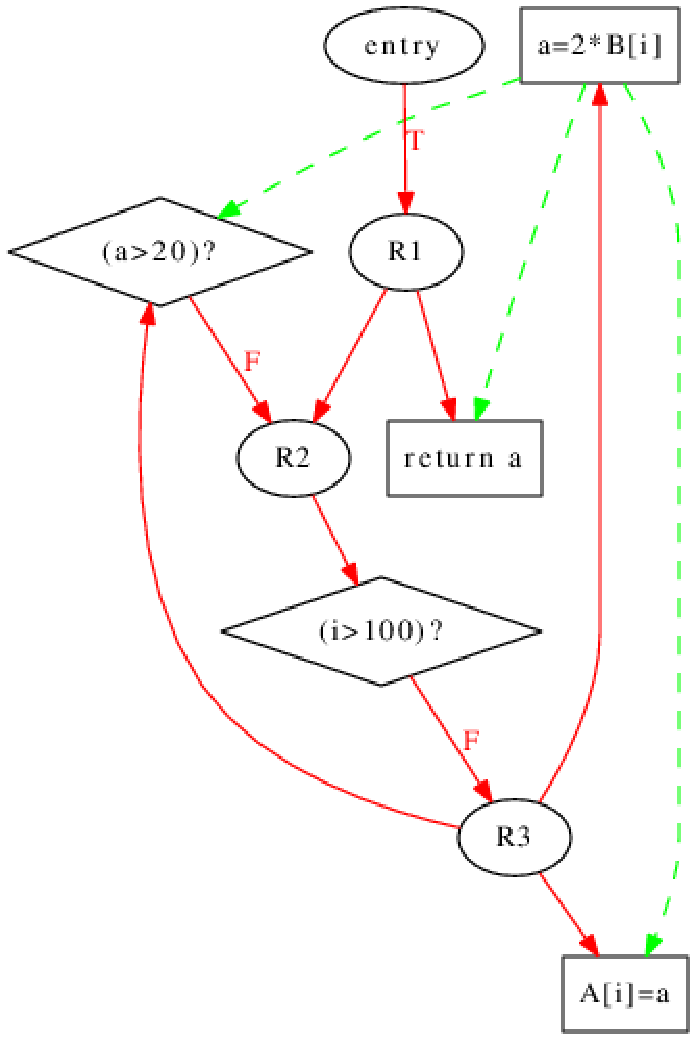
\includegraphics[scale=0.4]{pdg-2.pdf}
}
\caption{Some code translated into a PDG. Nodes associated with the evolution of the induction variable $i$ are omitted.}
\label{fig:pdg}
\end{figure}

Construction of the PDG is tackled in two steps from the CFG: 
construction of the control dependence subgraph and construction of the data dependence subgraph. 
The construction of the control dependence subgraph falls itself into two steps. 
First, control dependence between statements and predicate nodes are computed; 
then region nodes are added. 
A node $w$ is said to be \emph{control dependent on node $u$ along CFG edge $(u,v)$} or simply \emph{control dependent on edge $(u,v)$} if $w$ post-dominates $v$ and $w$ does not \emph{strictly} post-dominate $u$. 
Control dependence between nodes is nothing else than post-dominance frontier, i.e., dominance frontier on the reverse CFG. 
A slight difference in its construction process is that the corresponding control dependence edges from $u$ to $w$ is labeled by the boolean value taken by the predicate computed in $u$ when branching on edge $(u,v)$. 
To compute the control dependence subgraph, the post dominator tree is constructed for the procedure. 
Then, the $\texttt{ENTRY}$ node is added with one edge labeled {\sf true} pointing to the CFG entry node, and another labeled {\sf false} going to the CFG exit node. 
Then, let $S$ consist of all edges $(A,B)$ in the CFG such that $B$ is not an ancestor of $A$ in the post dominator tree. 
Each of these edges has an associated label {\sf true} or {\sf false}. 
Then, each edge in $S$ is considered in turn. 
Given $(A,B)$, the post dominator tree is traversed backwards from $B$ until we reach $A$'s parent, marking all nodes visited (including $B$) as control dependent on $A$ with the label of $S$.

Next, region nodes are added to the PDG. 
Each region node summarizes a set of control conditions and ``groups'' all nodes with the same set of control conditions together. 
Region nodes are also inserted so that predicate nodes will only have two successors. 
To begin with, an unpruned PDG is created by checking, for each node of the CFG, which control region it depends on. 
This is done by traversing the post dominator tree in post order, and using a hash table to map sets of control dependencies to region nodes. 
For each node $N$ visited in the post dominator tree, the hash table is checked for an existing region node with the same set $CD$ of control dependencies. 
If none exists, a new region node $R$ is created with these control dependencies and entered into the hash table. 
$R$ is made to be the only control dependence predecessor of $N$. 
Next, the intersection $INT$ of $CD$ is computed for each immediate child of $N$ in the post dominator tree. 
If $INT=CD$ then the corresponding dependencies are deleted from the child and replaced with a single dependence on the child's control predecessor. 
Then, a pass over the graph is made to make sure that each predicate node has a unique successor for each truth value. 
If more than one exists, the corresponding edges are replaced by a single edge to a freshly created region node that itself points to the successor nodes.

A statement $B$ that is to be executed after a statement $A$ in the original sequential ordering of the program depends on $A$ in the following situations: 
(flow) $B$ reads to a storage location that was lastly accessed by $A$ through a write; 
(anti) $B$ writes to a storage location previously accessed through a read by $A$; 
(output) $A$ and $B$ both have a write access to the same storage location. 
Side effects can also dictate the insertion of a dependence between $A$ and $B$ to force the sequential ordering of the final schedule. 
Memory accesses cannot always be analyzed with enough precision. 
In the presence of a may alias between two consecutive accesses, a conservative dependence is to be inserted also. 
Memory access locations often vary with the iterations of the enclosing loops. 
Dependence analysis can take advantage of some abstract representations of the access function such as when the memory address can be represented as an affine function of the induction variables. 
Not only does this enables a refinement of the alias information, but also the dependence can be labeled with a distance vector as a function itself of the loop indices. 
As an example, a loop indexed by $i$, that would access array $A[i]$ twice, first as a write at iteration $i$, then as a read at iteration $2i+1$, would lead to a flow dependence of distance $i+1$.
%FAB: Ferrante's paper is not very instructive to understand if there are some subtleties that should be understood. I actually do not find the discussion on the related work part very useful. One should read the work from Ottenstein that they refer to (I do not have access to it as I write this). The advantage of what you wrote is that is reports exactly what is written in Ferrante's paper, but it is very vague and seems to be restricted to some def-use chains. My current description, adheres with the understanding of Muchnich, that presents the dependence subgraph in the most classical way.  
%% DAGs are constructed for each basic block during the initial parse of the source program. Each upwards exposed use in a block has a corresponding DAG leaf node as usual; these leaves are called {\it merge nodes}. Data-flow analysis is then performed to compute the set of reaching definitions for each basic block, with the additional assumption that every variable is initially assigned the value ``undefined'' at program entry. Finally, the individual DAGs are connected to one another using the results of the data-flow computation: edges are added from definition nodes to the corresponding merge nodes that may be reached.

%FAB: I would suggest you put the corresponding references in the last section citing Harrold, but also the ``further improvements'' for generating sequential code that you talked about.
% I removed references to Harrold, Ferrante as it does not fit to the style of the book.
The PDG can also be constructed during parsing. 
Sequential code can be derived from a PDG, but generating the {\it minimal size} CFG from a PDG turns out to be an NP-Complete problem. 
The PDG's structure has been exploited for generating code for vectorisation, and has also been used in order to perform accurate program slicing and testing.

\subsection{Detecting parallelism with the PDG}

The structure of the PDG allows for parallelism to be detected easily. 
On a regular CFG representation, a scheduler based on data dependencies will generally restrict its scope to hyper-blocks. 
In this context, code transformations such as loop unrolling or if conversion (see Chapter~\ref{chapter:if_conversion}) that effectively change control dependencies into data dependencies can expose instruction level parallelism. 
However, the PDG can \textit{directly} be used to detect parallelism. 
As an example, any node of a CFG loop, that is not contained in an SCC of the PDG (considering \textit{both} control and data dependence edges) can be vectorized. 
In the example in Figure~\ref{fig:pdg}, since the statement \texttt{A[i]=a} in the loop do not form an SCC in the PDG, it can be vectorized provided array expansion of variable $a$. 
On the other hand, because of the circuit involving the test on $a$, the statement \texttt{a=2*B[i]} cannot.


\section{Gating functions and GSA}
\label{sec:gating_functions}
In SSA form, \phifuns are used to identify points where variable definitions converge. 
However, they cannot be directly \textit{interpreted}, as they do not specify the condition which determines which of the variable definitions to choose. 
By this logic, we cannot directly interpret the SSA Graph. 
Being able to interpret our IR is a useful property as it gives the compiler writer more information when implementing optimizations, and also reduces the complexity of performing code generation. 
Gated Single Assignment form (GSA; 
sometimes called Gated SSA) is an extension of SSA with \textit{gating functions}. 
These gating functions are directly interpretable versions of $\phi$-nodes, and replace $\phi$-nodes in the representation. 
We usually distinguish the three following forms of gating functions:

\begin{itemize}
\item The $\phiif$ function explicitly represents the condition which determines which $\phi$ value to select. 
  A $\phiif$ function of the form $\phiif(P,V_{1},V_{2})$ has $P$ as a predicate, and $V_{1}$ and $V_{2}$ as the values to be selected if the predicate evaluates to true or false respectively. 
  This can be read simply as \textit{if-then-else}.
\item The $\phientry$ function is inserted at loop headers to select the initial and loop carried values. A $\phientry$ function of the form $\phientry(V_{init},V_{iter})$, has $V_{init}$ as the initial input value for the loop, and $V_{iter}$ as the iterative input. We replace \phifuns at loop headers with $\phientry$ functions.
\item The $\phiexit$ function determines the value of a variable when a loop terminates. 
  A $\phiexit$ function of the form $\phiexit(P,V_{final})$ has $P$ as predicate and $V_{final}$ as the definition reaching beyond the loop.
\end{itemize}

\begin{figure}
\centering
\subfloat{
  \begin{minipage}[b]{0.3\linewidth}
    \texttt{\begin{tabbing}
        begin: \= i = 1;\\
        loop: \> if i > 100 goto end;\\
        \> a = 2 * B[i];\\
        \> A[i] = a;\\
        \> i = i + 1;\\
        \> if a > 20 goto end;\\
        \> goto loop;\\
        end: \> return a;\\
      \end{tabbing}}
  \end{minipage}
}
\subfloat{
  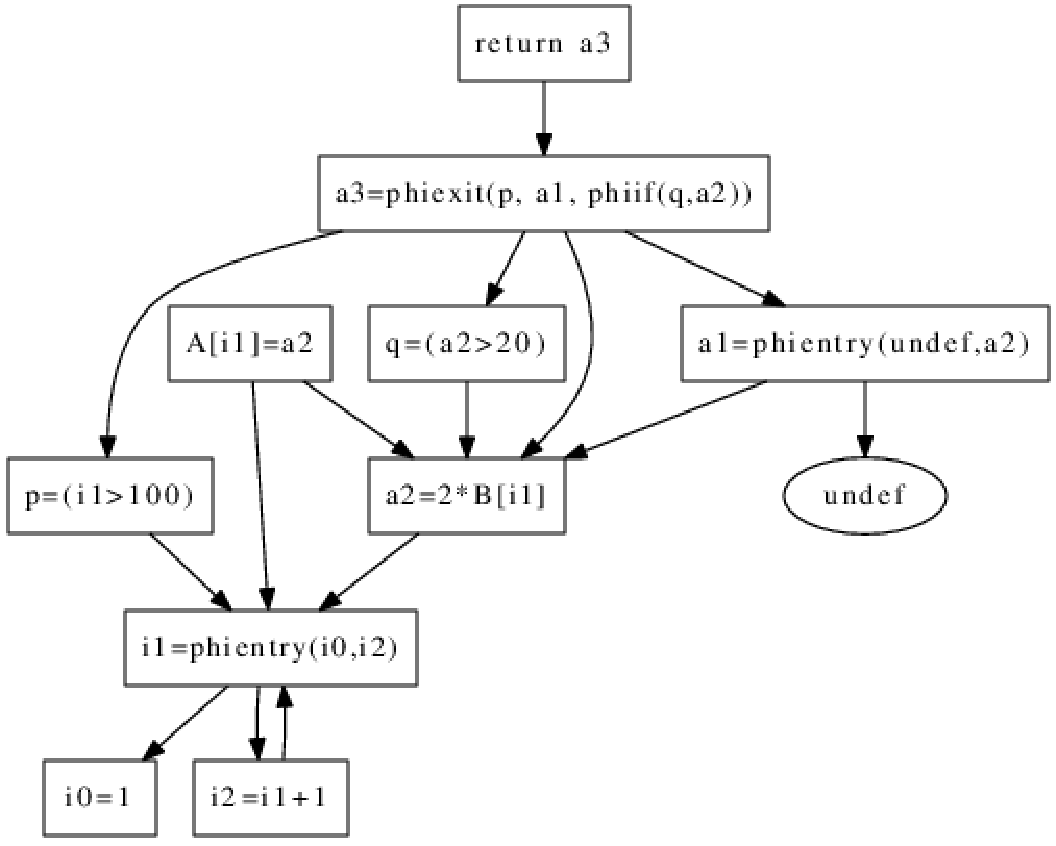
\includegraphics[scale=0.4]{gsa-example-2.pdf}
}
\caption{A graph representation of our sample code in GSA form.}
\label{fig: gsa-graph-example}
\end{figure}

It is easiest to understand these gating functions by means of an example. 
Figure~\ref{fig: 
  gsa-graph-example} shows how our earlier code in Figure~\ref{fig:pdg} translates into GSA form. 
Here, we can see the use of both $\phientry$ and $\phiexit$ gating functions. 
At the header of our sample loop, the \phifun has been replaced by a $\phientry$ function which determine between the initial and iterative value of $i$. 
After the loop has finished executing, the nested $\phiexit$ function selects the correct live-out version of $a$.

This example shows several interesting points. 
First, the semantic of both the $\phiexit$ and $\phiif$ are strict in their gate: 
here $a_1$ or $\phiexit(q,a_2)$ are not evaluated before $p$ is known~\footnote{As opposed to the $\psi$-function described in Chapter~\ref{chapter:psi_ssa} that would use syntax such as $a_3=\phi((p\wedge \lnot q)?a_1, (\lnot p\wedge q)?a_2)$ instead.}. 
Similarly, a $\phiif$ function that results from the nested if-then-else code of Figure~\ref{fig:vsdg:structured} would be itself nested as $a=\phiif(p,\phiif(q,a_2,a_3),a_1)$. 
Second, this representation of the program does not allow for an interpreter to decide whether an instruction with a side effect (such as $A[i_1]=a_2$ in our running example) has to be executed or not. 
Finally, computing the values of gates is highly related to the simplification of path expressions: 
in our running example $a_2$ should be selected when the path $\lnot p$ followed by $q$ (denoted $\lnot p . 
q$) is taken while $a_1$ should be selected when the path $p$ is taken; 
for our nested if-then-else example, $a_1$ should be selected either when the path $\lnot p . 
r$ is taken or when the path $\lnot p . 
\lnot r$ is taken which simplifies to $\lnot p$. 
Diverse approaches can be used to generate the correct nested $\phiif$ or $\phiexit$ gating functions.

\begin{figure}
\subfloat{
  \begin{minipage}[b]{0.3\linewidth}
    \texttt{\begin{tabbing}
        $a_1=...$\\
        if \= ($p$) then \\
        \> if ($q$) then ($a_2=...$)\\
        \> else ($a_3=...$)\\
        else\\ 
        \> if ($r$) then ($...$)\\ 
        \> else ($...$)
    \end{tabbing}}
  \end{minipage}
}
\subfloat{
  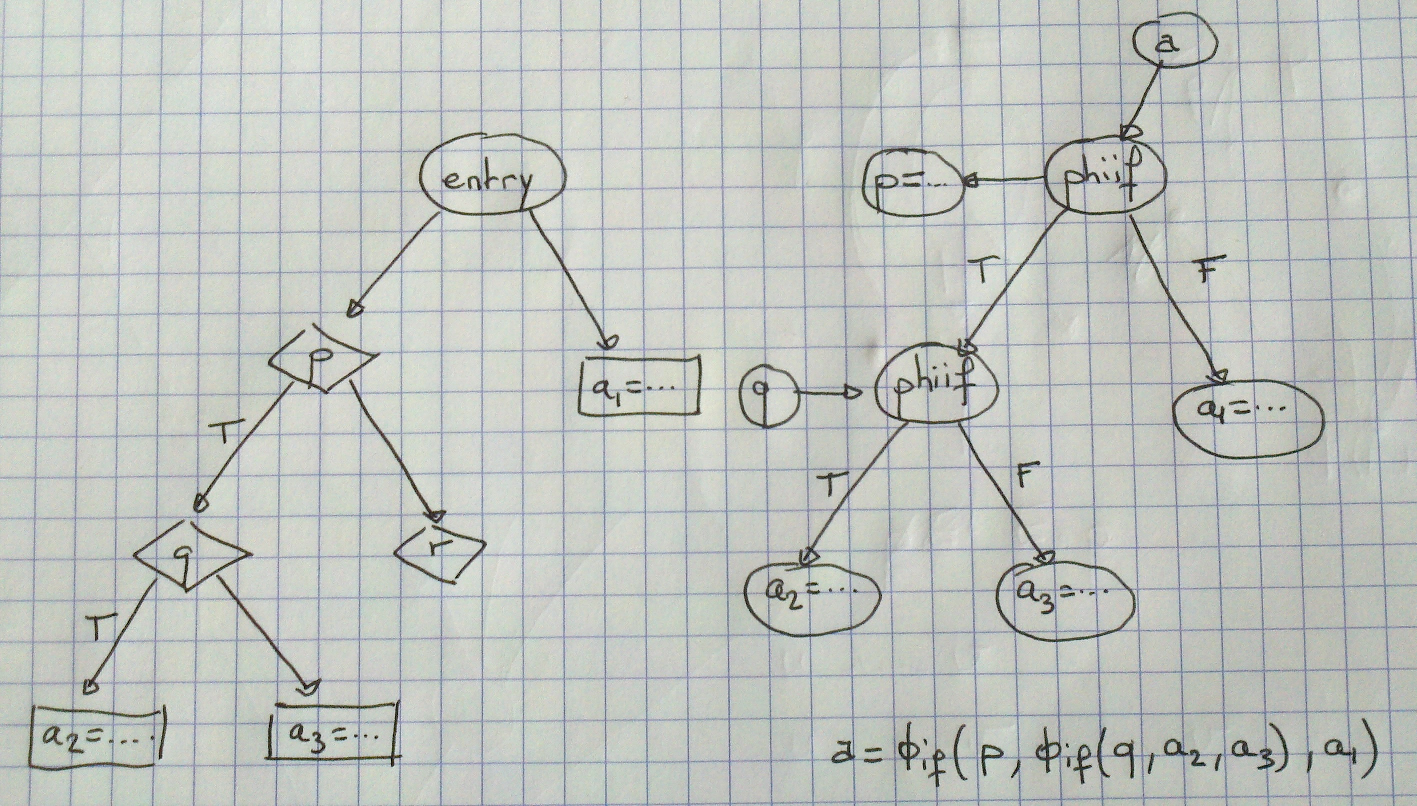
\includegraphics[width=0.6\textwidth]{cdg-structured.pdf}
}
\caption{(a) A structured code; (b) the CDG (with region nodes ommited); (c) the DAG representation of the nested gated $\phiif$ \label{fig:vsdg:structured}}
\end{figure}

The most natural way uses a data-flow analysis that computes, for each program points and each variable, its unique reaching definition and the associated set of reaching paths. 
This set of paths is abstracted using a \emph{path expression}. 
If the code is not already under SSA, and if at a merge point of the CFG its predecessor basic blocks are reached by different variables, a \phifun is inserted. 
The gates of each operand is set to the path expression of its corresponding incoming edge. 
If a unique variable reaches all the predecessor basic blocks, the corresponding path expressions are merged. 
Of course, a classical path compression technique can be used to minimize the number of visited edges. 
One can observe the similarities with the \phifun placement algorithm described in Section~\ref{section:alternative_ssa_construction_algorithms:loop}.

There also exists a relationship between the control dependencies and the gates: 
from a code already under strict and conventional SSA form, one can derive the gates of a $\phiif$ function from the control dependencies of its operands. 
This relationship is illustrated by Figure~\ref{fig:vsdg:structured} in the simple case of a structured code.
 
These gating functions are important as the concept will form components of the Value State Dependence Graph later. 
GSA has seen a number of uses in the literature including analysis and transformations based on data flow. 
With the diversity of applications (see chapters~\ref{chapter:hardware_compilation} and~\ref{chapter:loop_tree}), many variants of GSA have been proposed. 
Those variations concern the correct handling of loops in addition to the computation and representation of gates.


By using gating functions it becomes possible to construct IRs based solely on data dependencies. 
These IRs are sparse in nature compared to the CFG, making them good for analysis and transformation. 
This is also a more attractive proposition than generating and maintaining both a CFG and DFG, which can be complex and prone to human error. 
One approach has been to combine both of these into one representation, as is done in the PDG. 
Alternatively, we can utilize gating functions along with a data-flow graph for an effective way of representing whole program information using data-flow information.

\subsection{Backwards symbolic analysis with GSA}
GSA is useful for performing symbolic analysis. 
Traditionally, symbolic analysis is performed by forward propagation of expressions through a program. 
However, complete forward substitution is expensive and can result in a large quantity of unused information and complicated expressions. 
Instead, \textit{backward}, demand-driven substitutions can be performed using GSA which only substitutes \textit{needed} information. 
Consider the following program:

\begin{figure*}[ht]
\centering
\subfloat{
  \begin{minipage}[b]{0.3\linewidth}
    \texttt{\begin{tabbing}
        R: \= JMAX = Expr\\
        S: \> if(P) \= then J = JMAX - 1\\
           \> \> else J = JMAX\\
        T: \> $assert$(J ${\leq}$ JMAX)
      \end{tabbing}}
  \end{minipage}
}
\caption{A program on which to perform symbolic analysis.}
\label{fig:tupaduaexample}
\end{figure*}

If forward substitutions were to be used in order to determine whether the assertion is correct, then the symbolic value of \texttt{J} must be discovered, starting at the top of the program in statement \texttt{R}. 
Forward propagation through this program results in statement \texttt{T} being $assert((if $ $\texttt{P}$ $then$ $\texttt{Expr-1}$ $else$ $\texttt{Expr)}$ $\leq$ $\texttt{Expr}$ $\texttt{)}$, thus the \textit{assert} statement evaluates to true. 
In real, non-trivial programs, these expressions can get unnecessarily long and complicated.

Using GSA instead allows for backwards, demand-driven substitutions. The program above has the following GSA form:

\begin{figure*}
\centering
  \begin{minipage}[b]{0.3\linewidth}
    \texttt{\begin{tabbing}
        R: \= ${JMAX_1}$ = Expr\\
        S: \> if(P) \= then ${J_1}$ = ${JMAX_1}$ - 1\\
           \> \> else ${J_2}$ = ${JMAX_1}$\\
           \> ${J_3}$ = $\phiif$(P,${J_1}$,${J_2}$)\\
        T: \> $assert$(${J_3}$ ${\leq}$ ${JMAX_1}$)
      \end{tabbing}}
  \end{minipage}
\caption{Figure~\ref{fig:tupaduaexample} in GSA form.}
\label{fig:tupaduagsasubs}
\end{figure*}

Using this backwards substitution technique, we start at statement \texttt{T}, and follow the SSA links of the variables from ${J_3}$. 
This allows for skipping of any intermediate statements that do not affect variables in \texttt{T}. 
Thus the substitution steps are:

\begin{figure*}
\centering
  \begin{minipage}[b]{0.3\linewidth}
    \texttt{\begin{tabbing}
        ${J_3}$ = \= $\phiif$(P,${J_1}$,${J_2}$)\\
        \> = $\phiif$(P,${JMAX_1 - 1}$,${JMAX_1}$)
      \end{tabbing}}
  \end{minipage}
\caption{Substitution steps in backwards symbolic analysis.}
\label{fig:tuapaduagsaexample}
\end{figure*}

The backwards substitution then stops because enough information has been found, avoiding the redundant substitution of ${JMAX_1}$ by ${Expr}$. 
In non-trivial programs this can greatly reduce the number of redundant substitutions, making symbolic analysis significantly cheaper.

\section{Value State Dependence Graph}

The gating functions defined in the previous section were used in the development of a sparse data-flow graph IR called the Value State Dependence Graph (VSDG). 
The VSDG is a directed graph consisting of operation nodes, loop and merge nodes together with value and state dependency edges. 
Cycles are permitted but must satisfy various restrictions. 
A VSDG represents a single procedure: 
this matches the classical CFG.

An example VSDG is shown in Figure~\ref{fig:fac}. 
In (a) we have the original C source for a recursive factorial function. 
The corresponding VSDG (b) shows both value and state edges and a selection of nodes.

\begin{figure}[!htb]
\centering
\begin{tabular}{ccc}	%\cline{1-1}
\begin{minipage}[c][\height][t]{2.2in}
\texttt{\begin{tabbing}
int \=fac(int n) \{\\
\> int result;\\
\> if(\=n == 1)\\
\> \> result = n;\\
\> else\\
\> \> result = n * fac(n - 1);\\
\> return result;\\
\}
\end{tabbing}}
\end{minipage}
& \hspace{0.25in} &
\begin{minipage}[c][\height][b]{2.2in}
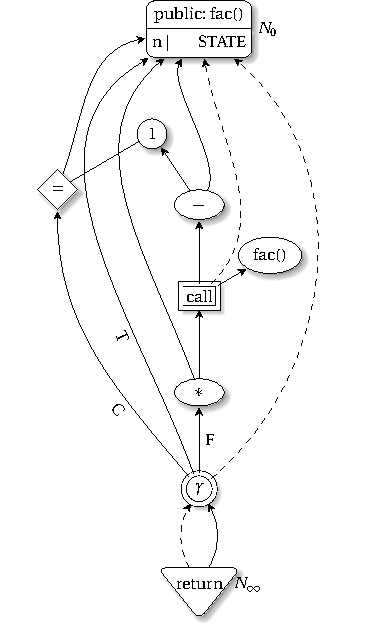
\includegraphics[scale=0.5]{example-fac}
\end{minipage}	\\ Ê%\cline{1-1}
& & \\
(a) & & (b)	\\ 
\end{tabular}

\caption{A recursive factorial function, whose VSDG illustrates the key graph components---value dependency edges (solid lines), state dependency edges (dashed lines), a \instruction{const} node, a \instruction{call} node, a \Gn, a conditional node, and the function entry and exit nodes.}
\label{fig:fac}
\end{figure}

%%%%%%%%%%%%%%%%%%%%%%%%%%%%%%%%%%%%%%%%%%%%%%%%%%%%%%%%%%%%%%%%%%%%%%%%%%%%%%%%

\subsection{Definition of the VSDG}

A VSDG is a labeled directed graph $G=(N,E_V,E_S,\ell,N_0,N_\infty)$ consisting of nodes $N$ (with unique entry node $N_0$ and exit node $N_\infty$), value dependency edges $E_V \subseteq N \times N$, state dependency edges $E_S \subseteq N \times N$. 
The labelling function $\ell$ associates each node with an operator.

The VSDG corresponds to a reducible program, e.g.~there are no cycles in the VSDG except those mediated by $\theta$ (loop) nodes.

Value dependency ($E_V$) indicates the flow of values between nodes. 
State dependency ($E_S$) represents two things; 
the first is essential sequential dependency required by the original program, e.g.~a given \texttt{load} instruction may be required to follow a given \texttt{store} instruction without being re-ordered, and a \texttt{return} node in general must wait for an earlier loop to terminate even though there might be no value-dependency between the loop and the \texttt{return} node. 
The second purpose is that state dependency edges can be added incrementally until the VSDG corresponds to a unique CFG. 
Such state dependency edges are called {\em serializing} edges.

The VSDG is implicitly represented in SSA form: 
a given operator node, $n$, will have zero or more $E_V$-consumers using its value. 
Note that, in implementation terms, a single register can hold the produced value for consumption at all consumers; 
it is therefore useful to talk about the idea of an output {\em port} for $n$ being allocated a specific register, $r$, to abbreviate the idea of $r$ being used for each edge $(n_1,n_2)$ where $n_2 \in \textit{succ}(n_1)$.
%Similarly, we will talk about (say) the
%``right-hand input port'' of a subtraction instruction, or of the $R$-input of
%a \Tn.

%%%%%%%%%%%%%%%%%%%%%%%%%%%%%%%%%%%%%%%%%%%%%%%%%%%%%%%%%%%%%%%%%%%%%%%%%%%%%%%%
%%
%%		NODE PROPERTIES
%%
%%%%%%%%%%%%%%%%%%%%%%%%%%%%%%%%%%%%%%%%%%%%%%%%%%%%%%%%%%%%%%%%%%%%%%%%%%%%%%%%

\subsection{Nodes}
There are four main classes of VSDG nodes: 
value nodes (representing pure arithmetic), \Gns\ (conditionals), Ê\Tns\ (loops), and state nodes (side effects). 
The majority of nodes in a VSDG generate a value based on some computation (add, subtract, etc.) applied to their dependent values (constant nodes, which have no dependent nodes, are a special case).


%%%%%%%%%%%%%%%%%%%%%%%%%%%%%%%%%%%%%%%%%%%%%%%%%%%%%%%%%%%%%%%%%%%%%%%%%%%%%%%

\subsection{$\gamma$-Nodes}

The \Gn\ is similar to the $\phiif$ gating function in being dependent on a control predicate, rather than the control-independent nature of SSA \phifuns.
%

A \Gn\ $\gamma(C, T, F)$ evaluates the condition dependency $C$, and returns the value of $T$ if $C$ is true, otherwise $F$.

%
We generally treat \Gns\ as single-valued nodes (contrast \Tns, which are treated as tuples), with the effect that two separate \Gns\ with the same condition can be later combined into a tuple using a single test. 
Figure~\ref{fig:twinPhis} illustrates two \Gns\ that can be combined in this way. 
Here, we use a pair of values (2-tuple) of values for the $T$ and $F$ ports. 
We also see how two syntactically different programs can map to the same structure in the VSDG.

\begin{figure}[!hb]
\centering
\begin{tabular}{ccc}	\cline{1-1}
\begin{minipage}[l]{2.0in}
\begin{verbatim}

a) ÊÊif (P)
ÊÊÊÊÊÊÊÊx = 2, y = 3;
ÊÊÊÊelse
ÊÊÊÊÊÊÊÊx = 4, y = 5;

b) ÊÊif (P) x = 2; else x = 4;
ÊÊÊÊÊÊÊ...
ÊÊÊÊif (P) y = 3; else y = 5;

\end{verbatim}
\end{minipage}	
& \hspace {0.2in}
\begin{minipage}[m][\height][l]{1.6in}
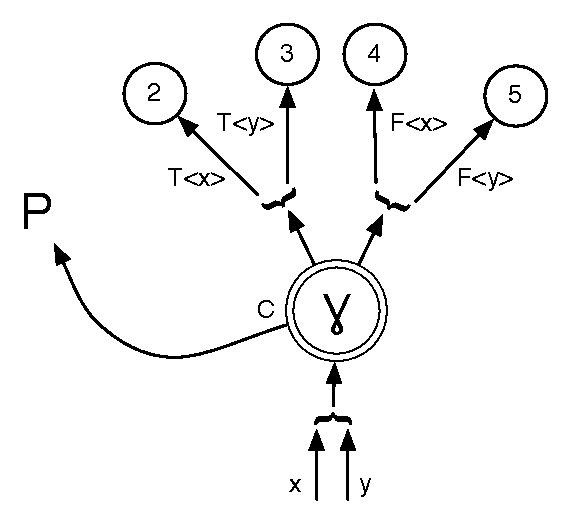
\includegraphics[scale=0.5]{vsdg-gammanodes}
\end{minipage} \\ \cline{1-1}
\end{tabular}

\caption{Two different code schemes (a) \& (b) map to the same
\Gn\ structure.}

\label{fig:twinPhis}
\end{figure}

%%%%%%%%%%%%%%%%%%%%%%%%%%%%%%%%%%%%%%%%%%%%%%%%%%%%%%%%%%%%%%%%%%%%%%%%%%%%%%%%

\subsection{$\theta$-Nodes}

The \Tn\ models the iterative behavior of loops, modeling loop state with the notion of an \emph{internal value} which may be updated on each iteration of the loop. 
It has five specific ports which represent dependencies at various stages of computation. 
The \Tn\ corresponds to a merge of the $\phientry$ and $\phiexit$ nodes in Gated SSA.
%

A \Tn\ $\theta(C,I,R,L,X)$ sets its internal value to initial value $I$ then, while condition value $C$ holds true, sets $L$ to the current internal value and updates the internal value with the repeat value $R$. 
When $C$ evaluates to false computation ceases and the last internal value is returned through the $X$ port.

%
A loop which updates $k$ variables will have: 
a single condition port $C$, initial-value ports $I_1,\ldots,I_k$, loop iteration ports $L_1,\ldots,L_k$, loop return ports $R_1,\ldots,R_k$, and loop exit ports $X_1,\ldots,X_k$. 
The example in Figure~\ref{fig:thetatuple} also shows a pair (2-tuple) of values being used for $I,R,L,X$, one for each loop-variant value.

% For some purposes the $L$ and $X$ ports could be fused,
% as both represent outputs
% within, or exiting, a loop (the values are identical, while the $C$ input
% merely selects their routing). ÊWe avoid this for two reasons:
% ({\it i\/}) we have operational semantics for VSDGs $G$
% and these semantics require separation of these concerns; and
% ({\it ii\/}) our construction of $G^\textit{noloop}$ requires it.

\begin{figure}[!ht]
\centering
\begin{tabular}{cc} \cline{1-1}
\begin{minipage}[c][\height][t]{0.9in}
\begin{verbatim}
j = ...
for(i = 0; 
i < 10; 
++i)
ÊÊÊ--j;
	
... = j;
\end{verbatim}
\end{minipage}
&
\begin{minipage}[c][\height][b]{3.0in}
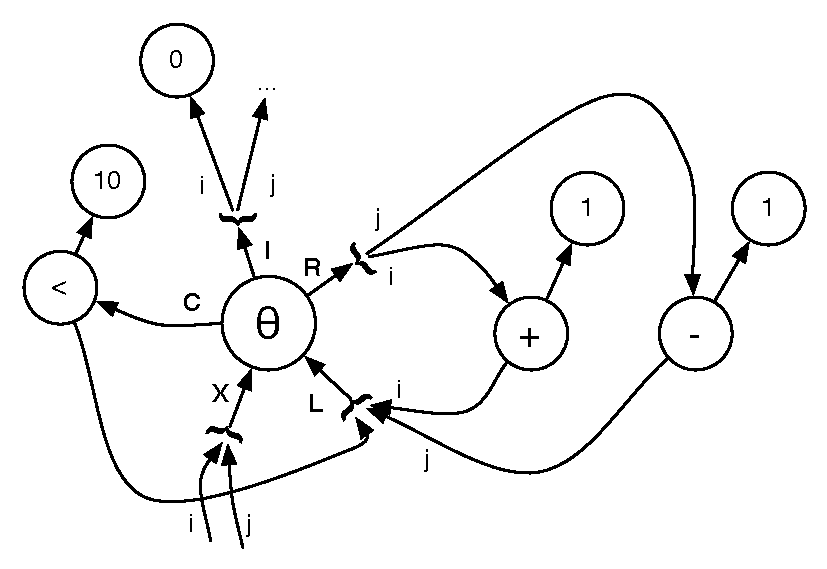
\includegraphics[scale=0.6]{vsdg-theta}
\end{minipage} \\ \cline{1-1}
\end{tabular}

\caption{An example showing a \texttt{for} loop. 
  Evaluating the \textbf{X} port triggers it to evaluate the \textbf{I} value (outputting the value on the \textbf{L} port). 
  While \textbf{C} evaluates to true, it evaluates the \textbf{R} value (which in this case also uses the $\theta$-node's \textbf{L} value). 
  When \textbf{C} is false, it returns the final internal value through the \textbf{X} port. 
  As \texttt{i} is not used after the loop there is is no dependency on the \texttt{i} port of \textbf{X}.}
\label{fig:thetatuple}
\end{figure}

The \Tn\ directly implements pretest loops (\instruction{while}, \instruction{for}); 
post-test loops (\instruction{do...while}, \instruction{repeat...until}) are synthesized from a pre-test loop preceded by a duplicate of the loop body. 
At first this may seem to cause unnecessary duplication of code, but it has two important benefits: 
({\it i\/}) it exposes the first loop body iteration to optimization in post-test loops (cf. 
loop-peeling), and ({\it ii\/}) it normalizes all loops to one loop structure, which both reduces the cost of optimization, and increases the likelihood of two schematically dissimilar loops being isomorphic in the VSDG.

%%%%%%%%%%%%%%%%%%%%%%%%%%%%%%%%%%%%%%%%%%%%%%%%%%%%%%%%%%%%%%%%%%%%%%%%%%%%%%%%

\subsection{State Nodes}
Loads and stores compute a value and state. 
The \instruction{call} node takes both the name of the function to call and a list of arguments, and returns a list of results; 
it is treated as a state node as the function body may read or update state.

\medskip

We maintain the simplicity of the VSDG by imposing the restriction that \emph{all} functions have \emph{one} return node (the exit node $N_\infty$), which returns at least one result (which will be a state value in the case of \instruction{void} functions). 
To ensure that function calls and definitions are able to be allocated registers easily, we suppose that the number of arguments to, and results from, a function is smaller than the number of physical registers---further arguments can be passed via a stack as usual.

Note also that the VSDG neither forces loop invariant code into nor out-of loop bodies, but rather allows later phases to determine, by adding serializing edges, such placement of loop invariant nodes for later phases.

\subsection{Dead node elimination with the VSDG}
By representing a program as a VSDG, many optimizations become trivial. 
For example, consider dead node elimination (Figure~\ref{fig:dnevsdg}). 
This combines both dead code elimination and unreachable code elimination. 
Dead code generates VSDG nodes for which there is no value or state dependency path from the \texttt{return} node, i.e., the result of the function does not in any way depend on the results of the dead nodes. 
Unreachable code generates VSDG nodes that are either dead, or become dead after some other optimization. 
Thus, a \textit{dead node} is a node that is not post dominated by the exit node $N_{\infty}$. 
To perform dead node elimination, only two passes are required over the VSDG resulting in linear runtime complexity: 
one pass to identify all of the live nodes, and a second pass to delete the unmarked (i.e., dead) nodes. 
It is safe because all nodes which are deleted are guaranteed never to be reachable from the \texttt{return} node.

\begin{figure}[!ht]
\centering
\begin{minipage}[t]{5in}
\noindent{\bf Input:} A VSDG $G(N,E_V,E_S,N_{\infty})$ with zero or more dead nodes.\\
\noindent{\bf Output:} A VSDG with no dead nodes.
\setcounter{linectr}{0}

Procedure DNE($G$) \{
\begin{code}
\x1 WalkAndMark($N_{\infty},G$);
\x1 DeleteMarked($G$);
\end{code}
\}

\setcounter{linectr}{0}
Procedure WalkAndMark($n,G$) \{
\begin{code}
\x1 {\bf if} $n$ is marked {\bf then} finish;
\x1 mark $n$;
\x1 {\bf foreach} (node $m \in N \wedge (n,m) \in (E_V \cup E_S)$) {\bf do}
\x2    WalkAndMark($m$);
\end{code}
\}

\setcounter{linectr}{0}
Procedure DeleteMarked($G$) \{
\begin{code}
\x1 {\bf foreach} (node $n \in N$) {\bf do}
\x2    {\bf if} $n$ is unmarked {\bf then} $delete$($n$);
\end{code}
\}

\end{minipage}
\caption{Dead node elimination on the VSDG.}
\label{fig:dnevsdg}
\end{figure}

%\section{Summary}
\section{Further readings}
A compiler's intermediate representation can be a graph, and many different graphs exist in the literature. 
We can represent the control flow of a program as a Control-Flow Graph (CFG)~\cite{808479}, where straight-line instructions are contained within basic blocks and edges show where the flow of control may be transferred to once leaving that block. 
A CFG is traditionally used to convert a program to SSA form~\cite{115320}. 
We can also represent programs as a type of Data-flow Graph (DFG)~\cite{dennis74first,dennis80data}, and SSA can be represented in this way as an SSA Graph~\cite{504710}. 
An example was given that used the SSA Graph to detect a variety of induction variables in loops~\cite{143131,201003}. 
It has also been used for performing instruction selection techniques~\cite{1375663,1269857}, operator strength reduction~\cite{504710}, rematerialization~\cite{143143}, and has been combined with an extended SSA language to aid compilation in a parallelizing compiler~\cite{Stoltz_extendedssa}.

% cite Harrold.
The Program Dependence Graph (PDG) as defined by Ferrante et al.~\cite{ferrante87the} represents control and data dependencies in one graph. 
Their definition of control dependencies that turns out to be equivalent to the post-dominance frontier leads to confusions at it uses a non-standard definition of post-dominance. 
We choose to report the definition of Bilardi and Pingali~\cite{Bilardi1996}. 
Section~\ref{section:vsdg:pdg} mentions possible abstractions to represent data dependencies for dynamically allocated objects. 
Among others, the book of Darte et al.~\cite{DarteRV-book} provides a good overview of such representations. 
The PDG has been used for program slicing~\cite{ottenstein84program}, testing~\cite{bates93incremental}, and widely for parallelization~\cite{ferrante85on,ferrante88generating,simons90a,baxter89program}. 
We showed an example of how the PDG directly exposes parallel code.

Gating functions can be used to create directly interpretable \phifuns. 
These are used in Gated Single Assignment Form. 
Alpern et al.~\cite{AlpernWZ88} presented a precursor of GSA for structured code, to detect equality of variables. 
This chapter adopts their notations, i.e., a $\phiif$ for a if-then-else construction, a $\phientry$ for the entry of a loop, and a $\phiexit$ for its exit. 
The original usage of GSA was by Ballance et al.~\cite{93578} as an intermediate stage in the construction of the Program Dependence Web IR. 
Further GSA papers replaced $\phiif$ by $\gamma$, $\phientry$ by $\mu$, and ~$\phiexit$ by $\eta$. 
Havlak~\cite{Havlak93constructionof} presented an algorithm for construction of a simpler version of GSA---Thinned GSA---which is constructed from a CFG in SSA form. 
The construction technique sketched in this chapter is developed in more detail in~\cite{207115}. 
GSA has been used for a number of analyses and transformations based on data flow. 
The example given of how to perform backwards demand-driven symbolic analysis using GSA has been borrowed from~\cite{tu95gated}. 
If conversion (see Chapter~\ref{chapter:if_conversion}), converts control dependencies into data dependencies. 
To avoid the potential loss of information related to the lowering of \phifuns into conditional moves or select instructions, gating $\psi$-functions (see Chapter~\ref{chapter:psi_ssa}) can be used.

We then described the Value State Dependence Graph (VSDG)~\cite{UCAM-CL-TR-607}, which is an improvement on a previous, unmentioned graph, the Value Dependence Graph~\cite{177907}. 
It uses the concept of gating functions, data dependencies and state to model a program. 
We gave an example of how to perform dead node elimination on the VSDG. 
Detailed semantics of the VSDG are available~\cite{UCAM-CL-TR-607}, as well as semantics of a related IR: 
the Gated Data Dependence Graph~\cite{upton}. 
Further study has taken place on the problem of generating code from the VSDG~\cite{DBLP:conf/pdpta/Upton03,UCAM-CL-TR-705,stanier11thesis}, and it has also been used to perform a combined register allocation and code motion algorithm~\cite{Johnson_combinedcode}.
